\chapter{Alternative methods}
\label{chap:alternative}
\section{Alternative Methods Considered}
\label{sec:alternative}
Being able to record simultaneously from multiple neurons allows us to investigate the effect of changes in a single neuron on a complete circuit. Such recordings could also give insight into the effect of modulators on individual neurons in a circuit but with the added advantage that differential changes in each neuron can be captured simultaneously.

Traditional electrophysiological techniques, such as the use of glass micro-electrodes and wire electrodes, have limitations. The main limitation being the physical size of the equipment when working on microscopic biological preparations.

As part of this research we investigated the use of alternative dyes , alternative delivery of dyes and alternative ways of recording:

\section{Voltage Sensitive Dyes}
\subsection{Methods}
\label{sec:alternative_vsd}
The use of \acp{VSD}, especially if bath-applied, allow us to record form multiple neurons. When used on the \ac{STG} we have been able to isolate signals for as many as 19 inidividual neurons. \acp{VSD} do however have some drawbacks that justifies further research into the development of dyes that would provide better signal to noise ratios, higher responsivity and lower toxicity.

As part of this research, pilot work was done to investigate \ac{VSD} design. Five newly designed\footnote{The dyes were developed in collaboration with Prof. Andrew C. Benniston at the Molecular Photonics Laboratory, School of Chemistry, Newcastle University, Newcastle upon Tyne NE1 7RU, UK} \acp{VSD} were tested (MJULBD, JULBD, AN024, AN192, NMACr) of which the results from two of the dyes, JULBD and MJULBD, were promising enough to be published in a journal paper. The dyes are low molecular weight julolidine-based borondipyrromethene (Bopidy) dyads \cite{Bai2014}. 

Protocols for recording with the new dyes were similar to that used with Di-4 ANEPPS which was discussed in section \ref{sec:vsd}. 5$mg$ of Bodipy dye was dissolved in 1$ml$ DMSO that contains 20\% pluronic acid. A 20 $\mu l$ sample of the stock se-olution was then dissolved in crab saline to obtain $10^{-5}$, $10^{-4}$ and $10^{-3}$ solutions. A petroleum jelly well was made around the \ac{STG} and filled with the dye solution to bathe the \ac{STG} for approximately 20 minutes. The dye was then washed away with a flowing saline solution before imaging (figure \ref{fig:julbdstain}).

\begin{figure}[H]
	\begin{center}
		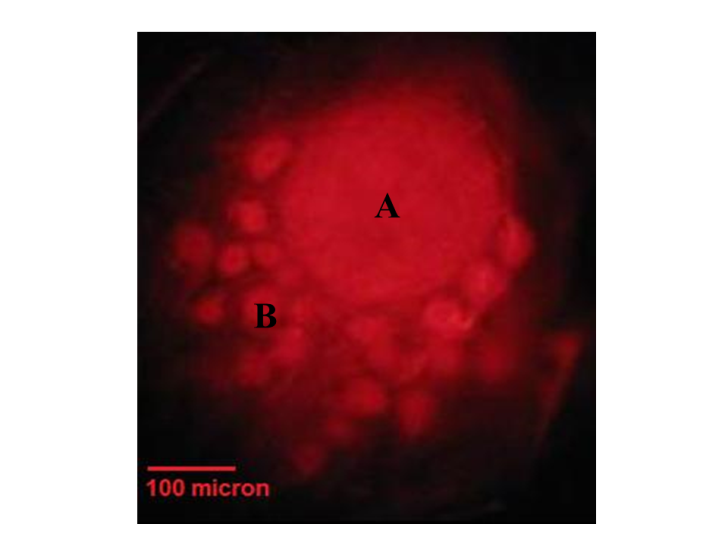
\includegraphics[width=\columnwidth]{graphics/julbdstain.png}
		\caption[Fluorescence image of the stomatogastric ganglion (STG)]{\textbf{Fluorescence image of the stomatogastric ganglion (STG)} of \species{Cancer pagurus} after bathing with a JULBD saline solution. (A) neuropil, (B) an STG neuron.}
		\label{fig:julbdstain}
	\end{center}
\end{figure}

\subsection{Results}
\footnote{These results were also published in \cite{Bai2014}}The sensitivity of the Bodipy dyes, MULBD and JULBD, were compared with that of di-4-ANEPPS. For the comparison, event-triggered averaging was carried out for recordings made with the Bodipy and di-4-ANEPPS dyes that clearly reflected neural activity . The dynamic range for MJULBD was 9.3\% of the di-4-ANEPPS dynamic range and for JULBD it was 30\%. Results shown in figure \ref{fig:julbdrecording} and figure \ref{fig:mjulbdrecording} show the imaging recordings matching the activity of a neuron that ws recorded using an intracellular electrode.

\begin{figure}[H]
	\begin{center}
		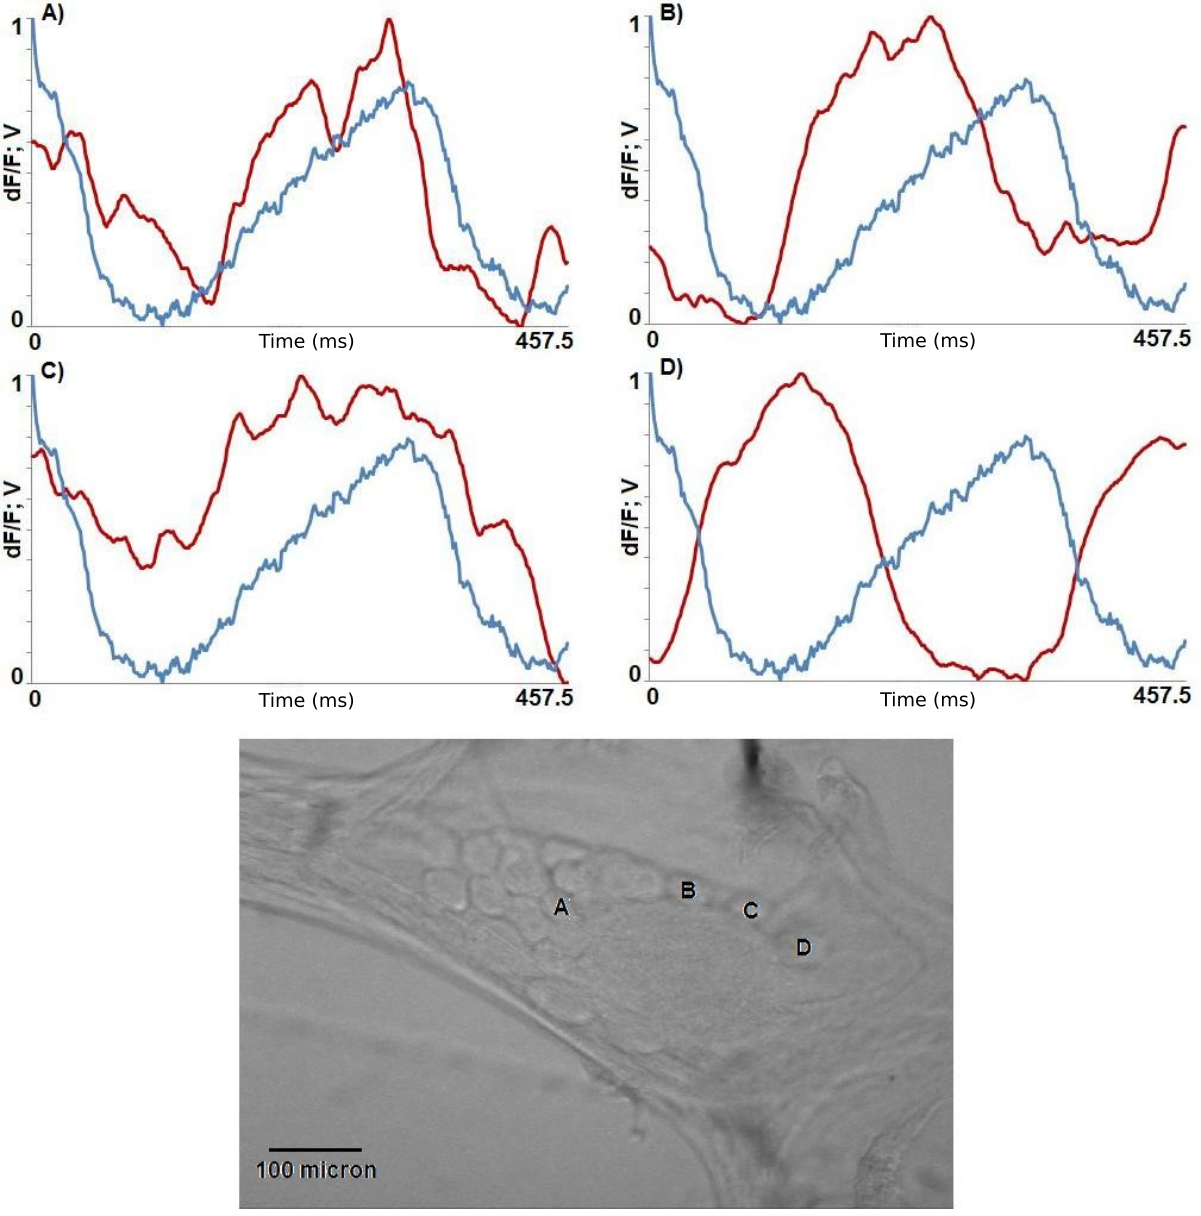
\includegraphics[width=\columnwidth]{graphics/julbdrecording.png}
		\caption[Intracellular and optical \ac{VSD} recording using JULBD of neural activities in the crab STG.]{\textbf{Intracellular and optical \ac{VSD} recording using JULBD of neural activities in the crab STG.} (A) \ac{PY} neuron recorded simultaneously by intracellular and optical \ac{VSD} recording; (B–D) other \ac{STG} neurons recorded only by \ac{VSD} imaging and considered against the reference provided by the intracellular recording of the \ac{PY} neuron shown in (A). The blue traces in all panels show the intracellular electrical recording of the \ac{PY} neuron. The red traces in all panels show the \ac{VSD} fluorescence imaging recording of the corresponding neurons marked in the bottom panel. All shown recording data were calculated using event-triggered averaging as described in the paper. The units on the vertical axes are arbitrary scaled units.}
		\label{fig:julbdrecording}
	\end{center}
\end{figure}
\begin{figure}[H]
	\begin{center}
		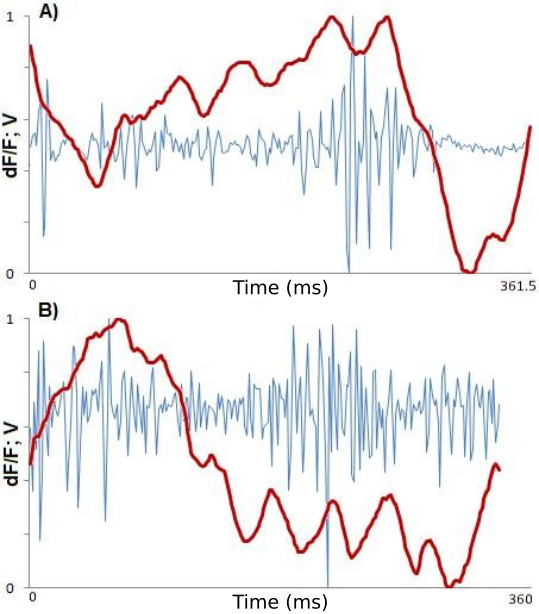
\includegraphics[width=12cm]{graphics/mjulbdrecording.png}
		\caption[Extracellular and optical \ac{VSD} recording using MJULBD of neural activities in the crab \ac{STG}]{\textbf{Extracellular and optical \ac{VSD} recording using MJULBD of neural activities in the crab \ac{STG}}. The blue traces in the panel shows the extracellular recording of full pyloric cycle from the \ac{lvn}. The red traces in the panel shows the \ac{VSD} imaging recording of an \ac{STG} neuron. All shown data were calculated using event-triggered averaging as described in section \ref{sec:detrend}. The units on the vertical axes are arbitrary scaled units}
		\label{fig:mjulbdrecording}
	\end{center}
\end{figure}

Also of interest when developing \acp{VSD} is toxicity. The toxic effect of \acp{VSD}, typically speeds up the pyloric rhythm. The toxic effects of the Bodipy dyes were compared to that of di-4-ANEPPS by measuring the impact of the dye on the pyloric rhythm cycle while the the \ac{STG} preparation was exposed to exciting illumination.

For the analysis recordings made with dye solutions of $10^{-5}$M dye concentration were used. It was found that there was a reduction of cycle length from one cycle to the next of 2.4\% for JULBD. Using a t-test at 5\% significance, this reduction proved to be significantly positive. di-4-ANEPPS and MJULBD however, showed no significant shortening of cycle length.

Over a long period, i.e. several minutes, all dyes prove to have some toxic effect which is reflected by the shortening rhythm cycle length.

\subsection{Discussion}
Zwitterionic dyes such as di-4-ANEPPS and di-8-ANEPPS are the dominating technology for \ac{VSD} imaging. There is, however, still room for improvement  with regards to toxicity, responsivity and signal to noise ratio.

As an alternative to zwitterionic voltage sensitive dyes we investigated the use of dyes based on the Bodipy framework for \ac{VSD} imaging. Our results are the first to demonstrate that Bodipy dyes can be used for neural imaging.

The MJULBD dye gives a much narrower dynamic range for the signal, but it has similar low toxicity as di-4-ANEPPS. Although the fluorescence voltage response of JULBD proved not to be any better than that of 4-ANEPPS, it appears that the BF$_{2}$ group reduces the toxicity of Bipody dyes to neurons \cite{Bai2014}.

\subsection{Conclusion}
The search for methods that would provide a better signal to noise ratio when recording neural activity is ongoing. It is also of vital importance to find methods that would allow the recording of whole networks as recordings from individual or a few neurons do not give sufficient information to understand complete networks. \Acp{VSD} offer a solution but there is still a great deal of research and development to be done to increase the signal to noise ratio and reduce the toxicity of such dyes.

The positive results from the pilot study has resulted in further funding being obtained from the Leverhulme Trust in the amount of ca. \pounds 170K. This study into the development of Bodipy dyes will be a partnership between the laboratories of Prof. Peter Andras from Keele University and Prof. Andrew Benniston from Newcastle University.

\section{Multi-electrode Arrays}
\subsection{Methods}
\label{subsec:MEA}

The possibility exists that \acp{MEA} can be used in conjunction with \acp{VSD}. Potentially simultaneously recording of neural activity with 
both  the \ac{MEA} and \ac{VSD} can be done. \acp{MEA} can also be used to stimulate neurons. Such stimulation would allow us to study the effect of stimulating specific neurons on the known rhythms produced by the central pattern generators found in the \ac{STG}. The main reason for considering the use of the \ac{MEA} and \ac{VSD} would be to overcome the restrictions of traditional electrophysiological methods to record activity of all the neurons of the \ac{STG} simultaneously. 

In collaboration with the laboratory of Prof. George Kemenes, from Sussex University, we investigated the use of a \ac{MEA} on the \ac{STG} of \species{Cancer pagurus}. The deafferented and desheathed \ac{STG} was placed on a \ac{MEA} with 252 electrodes which were 30 $\mu m$ in diameter and spaced 100 $mu$m apart. The nervous system was held in place by a combination of plastic strips, Blu Tack and a glass cover slip.

Neural activity was recorded using MC Rack software produced by MultiChannel Systems. Spike sorting was accomplished using a \matlab script which implements a a centre-of-mass calculation which is described in a paper by Novak and Wheeler \cite{Novak1986}. A 20 $\mu V$ threshold was used to detect spikes in 100Hz high-pass filtered data.

\subsection{Results}
Of six experiments done, the experiment which recorded the most active neural activity was chosen.  Using the  \matlab scripts mentioned in section \ref{subsec:MEA}, 33293 spikes were triangulated in the first 10 minutes of recording. A spike could be triangulated if it was detected on at least three electrodes at an amplitude of 20$\mu V$ or more. A typical recording over one electrode is shown in figure \ref{fig:MEA_recording}.

Figure \ref{fig:MEA_recording} shows a typical recording of the neural activity that was recorded over one electrode. A 5Hz rhythmic pattern can be observed in the recording. At least 23 spatially distinct spike sources were detected. These sources are shown in figure \ref{fig:MEA_analysis1a} and \ref{fig:MEA_analysis2}.

\begin{figure}[H]
	\begin{center}
		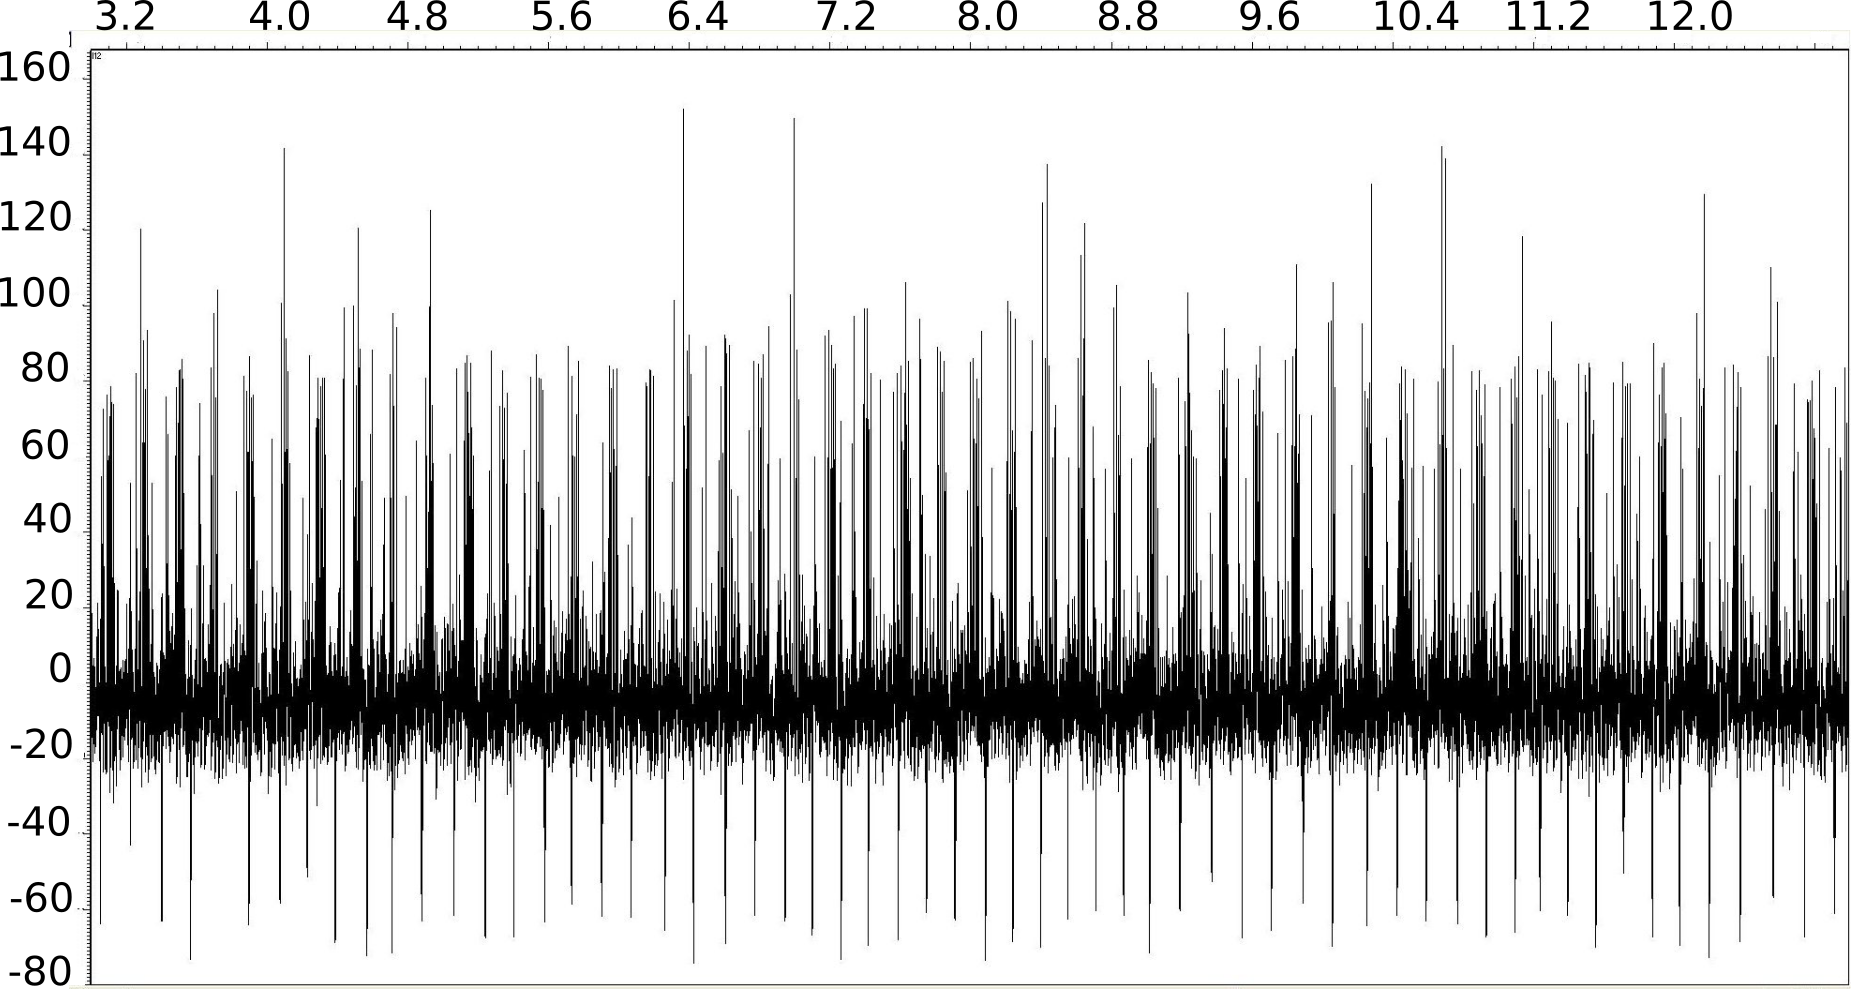
\includegraphics[width=13cm]{graphics/MEA_recording.png}
		\caption[\ac{MEA} Recording]{\textbf{MEA recording. }A typical recording of neural activity over one electrode as recorded with a multi-electrode array. A 5Hz rhythmic pattern could be observed.}
		\label{fig:MEA_recording}
	\end{center}
\end{figure}
\begin{figure}[H]
	\begin{center}
		\includegraphics[width=13cm]{graphics/MEA_analysis1a.png}
		\caption[\ac{MEA} Spike sources detected with a \matlab script.]{\textbf{\ac{MEA} Spike sources detected with a \matlab script.} Each detected spike is shown as circle. The detected spikes are overlaid on the image of the \ac{STG}, showing where on the \ac{STG} the spikes originated. The \acp{aln} and \ac{dvn} are labelled on the image. Figure \ref{fig:MEA_analysis2}, is an enlarged view of the activity.}
		\label{fig:MEA_analysis1a}
	\end{center}
\end{figure}
\begin{figure}[H]
	\begin{center}
		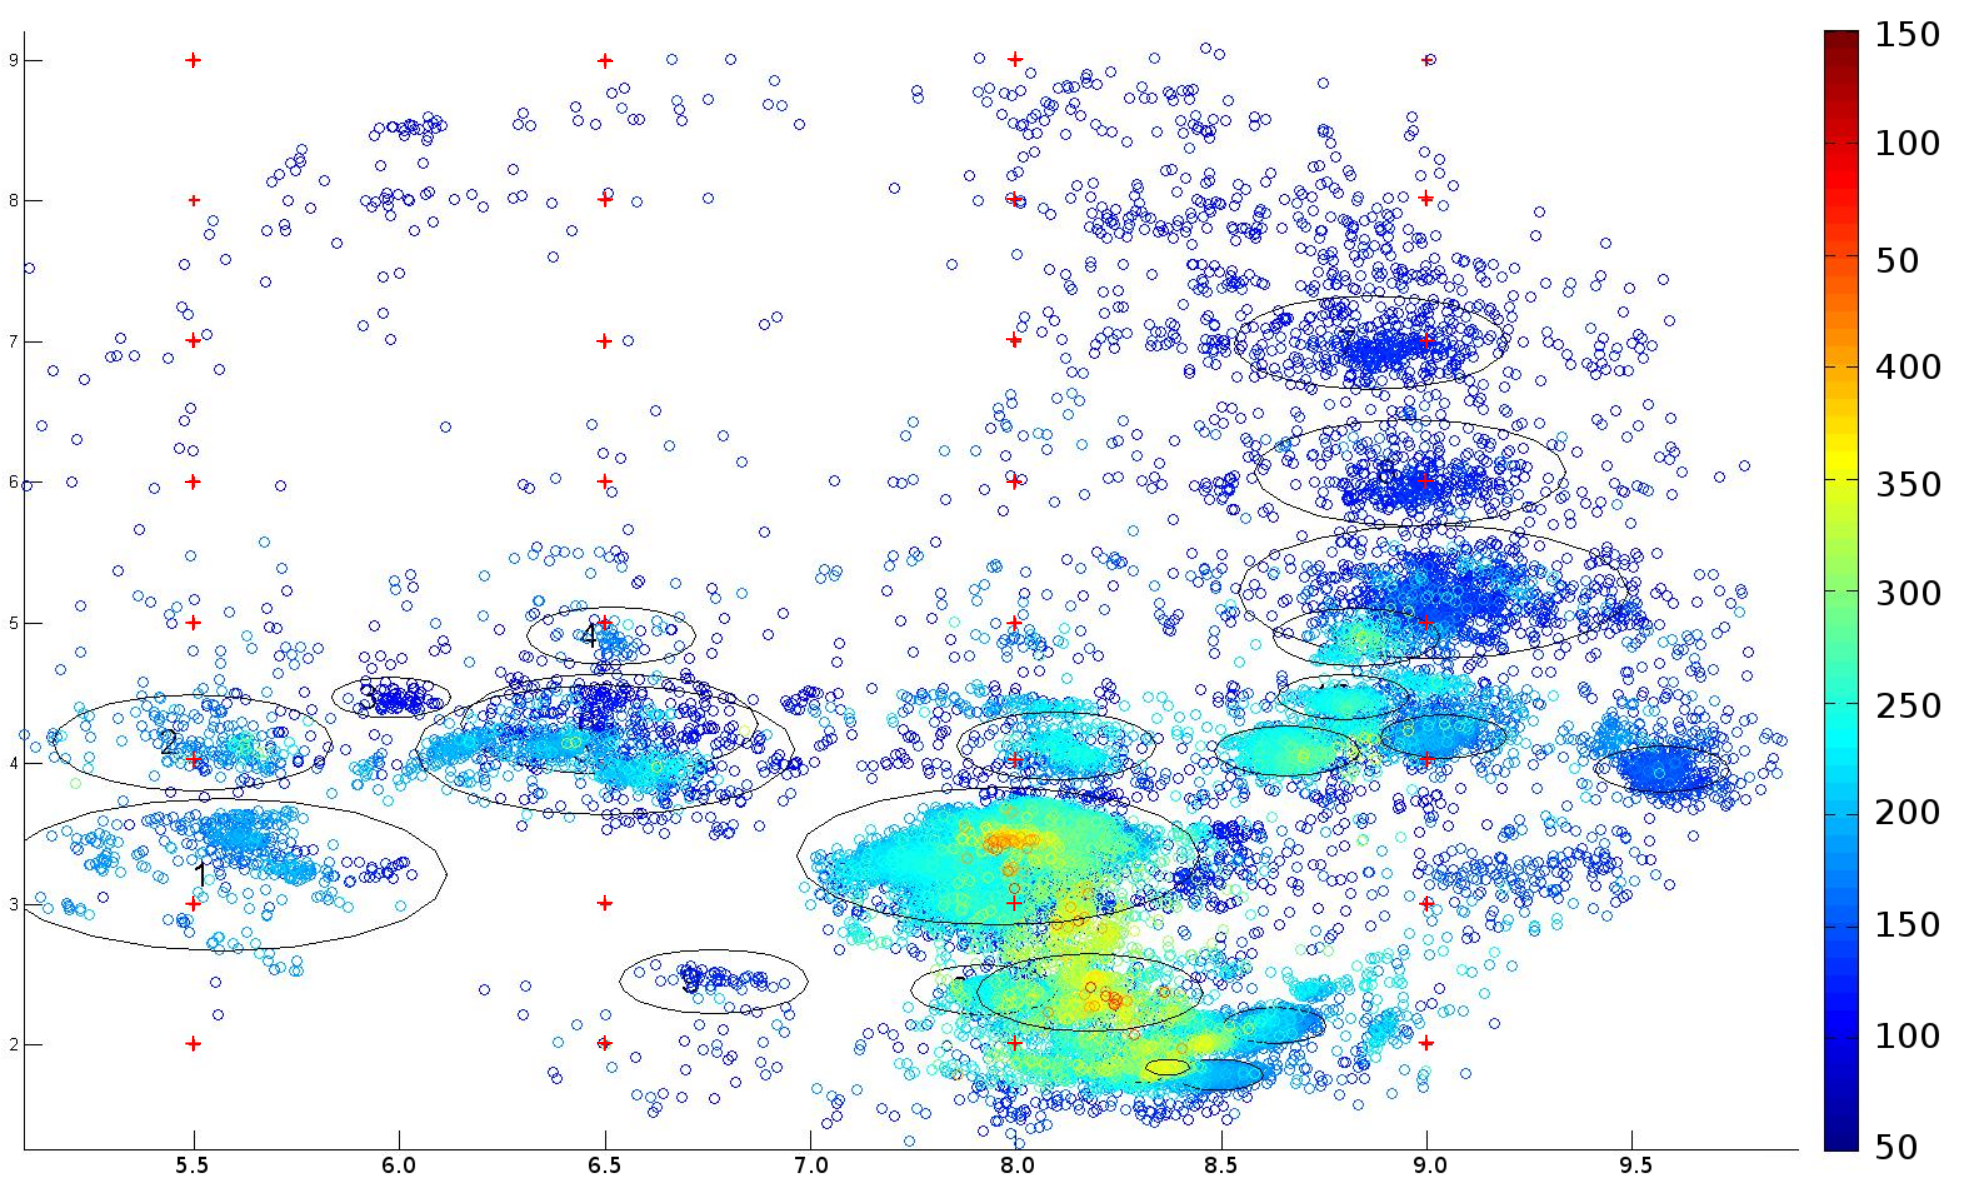
\includegraphics[width=\columnwidth]{graphics/MEA_analysis2a.png}
		\caption[Spike sources detected on \ac{MEA} recording. ]{\textbf{Spike sources detected on \ac{MEA} recording. }At least 23 spatially distinct spike sources were detected. The small red crosses on the image shows the position of the electrodes. Each circle is a spike that was detected in the first 10 minutes of the recording. The colour of the circle reflects a normalised amplitude of the spike.}
		\label{fig:MEA_analysis2}
	\end{center}
\end{figure}

\subsection{Discussion}
To provide insight into neural activity over the whole \ac{STG} we investigated the use of \acp{MEA} as a method of recording. It was found that most spikes and distinct areas of activity were identified over the neuropil which raised the question whether some areas might be neurite segments of the same neuron rather than neurons. To determine whether this is indeed the case further analysis will be required. It has been found that signals recorded over the neuropil are predominantly from the \acp{PD} but it is not possible to confirm whether this was the case with the recordings made for this initial investigation into the use of \acp{MEA}. The equipment used during the investigation, lacked the facility for making an extra-cellular recording which is usually used to identify the timing, and thus the identification of the spiking neuron.

The 5Hz rhythmic activity observed in figure \ref{fig:MEA_recording} was not evident in the spike sorted data. Re-sorting the data at a higher voltage threshold should resolve this discrepancy.

We have shown, however, that it is possible to successfully record from the \ac{STG} using an \ac{MEA}. In terms of hardware, software and protocols, areas were identified that will need refining to successfully use the \ac{MEA}, either independently or in conjunction with \ac{VSD}.

\note{pilot work in vsd design (mention more about our paper), mea and optogenetics.}

\note{How to design rationally the vsd. Basic boron module good for rational molecular design.}

\subsection{Conclusion}
With its added functionality of stimulation, \acp{MEA} could prove of significant value in research on the \ac{STG} as an alternative to \acp{VSD} or even for use in combination with \acp{VSD}. Both these methods allow recording from the whole \ac{STG}. Being able to study the effect of stimulation of one or more neurons or the effect of a modulation on all the neurons at the same time could give us invaluable insight into the workings of \acp{CPG}.

We have shown that we can successfully record from the \ac{STG} using an \ac{MEA}. We have identified areas, in terms of hardware, software and protocols, that will need refining to successfully use the \ac{MEA} in conjunction with \acp{VSD}. 

The equipment that were used for the proof of concept experiments, were from a \species{Lymnea stagnalis} lab, which were not adequately set up for \ac{STG} experiments. Perfusion of the preparation is required to keep the temperature of the saline between 10 and 15 degrees Celsius and can be implemented in the same manner as is used for \ac{VSD} and electrophysiological experiments.

Extra-cellular recordings are of vital importance to be able to identify spiking neurons that are being recorded. In the case of \ac{MEA} setup, a suction electrode has to be used rather than wire electrodes.


\section{Injection of dyes using compressed air}
\subsection{Methods}
\label{subsec:picospritzer}
Yet another method that was investigated is the use of compressed air to inject \ac{VSD} into cells. To our knowledge, this method has not been attempted before for the injection of \ac{VSD} into neurons. The Picospritzer III is a rack mountable system which can supply controlled and repeatable pressure pulses. Rather than using current to drive the dye into the cell, compressed air is pushed into a dye filled glass microelectrode. Glass microelectrodes are pulled as for intracellular recordings and dye fillings but the point of the microelectrode is broken off and polished, using an open flame, to obtain a slightly larger diameter. The electrode is then placed tightly against the cell, but not so that it penetrates the membrane. When the compressed air is pushed into the glass electrode, the dye is injected into the cell.

The glass microelectrodes were pulled using a P-97 Flaming/Brown Micropipette Puller from Sutter Instruments. The following settings on the puller were found to produce microelectrodes with the most appropriate shape with regards to taper and tip size for injection:

\begin{table}[H]
	\centering
	\label{tab:puller}
	\caption{Pipette Puller settings for microelectrodes used for injection with the Picospritzer.}
	\begin{tabular}{c c c c c}
		Ramp & Head & Pull & Velocity & Time/Del \\ \hline
		511 & 511 & 30 & 80 & 250
	\end{tabular}
\end{table}

The duration and pressure of the air injection of the dye is also important. After some experimentation we found the settings as shown in table \ref{tab:injection} to be ideal in that the dye was injected into the cell without damaging the neuron. The viability of the preparation during injection could be confirmed by make sure that the pyloric rhythm which is recorded during injection remains unaltered.

\begin{table}[H]
	\centering
	\caption{Picospritzer settings used for injection of \ac{VSD} into pyloric neurons.}
	\label{tab:injection}
	\begin{tabular}{c c}
		Duration (msec) & Pressure (PSI) \\ \hline
		500 & 30 
	\end{tabular}
\end{table}

\subsection{Results}
Because injection of \ac{VSD} with electrical pulses is so time consuming the neurons are usually identified first in order to fill only neurons specific to the requirements of the experiment. The preparation is not likely to survive the amount of time that would be required to inject all neurons with the electrical pulse method and then to be identified later with imaging data. Injection of \ac{VSD} using the Picospritzer III is an exciting prospect as it allows for instantaneous injection of dye which would otherwise take at least thirty minutes per neuron when using conventional intracellular injection with electrical pulses. It also allows for all visible neurons to be injected without having to identify neurons first as identification can be done afterwards from the imaging data.

Dye was successfully injected into several cells of the \ac{STG} with the cells surviving the injection and the pyloric rhythm maintained. The process of injecting the dye into several cells took less than an hour. It was thus shown that it is also possible to inject many cells in a short period. As many cells as can be seen can be filled to allow recording from as many cells as possible. Avoiding the penetration of cells multiple times (first for identification and then for filling) also reduces the risk of damaging the preparation. 

\subsection{Discussion}
Time did not allow for the refinement of the process for injecting \ac{VSD} using compressed air. However, it was shown in principle that the method should work and possibly provide a much better alternative for filling cells with intracellular \ac{VSD}. Intracellular \ac{VSD} has the advantage of giving a much better signal to noise ratio for better recording of neural activity but the skill required and the amount of time it takes to first identify and then fill a neuron using electrical pulses makes it a very difficult method to use. Injection using compressed air could potentially provide a much easier and quicker method with better results.

\subsection{Conclusion}
The fact that injection with compressed air can be successfully used as a delivery mechanism on neurons of the \ac{STG}, opens up other possibilities such as optogenetics. Optogenetics is already used successfully in model organisms such as \textit{Caenorhabditis elegans} \cite{Husson2013} and \textit{Danio rerio} \cite{DelBene2012}. In these two species genetically altered strains of the organisms are bread for experimentation. In crustacean however, this would not necessarily be an option because these animals take about four years to reach the required size. On the other hand it is possible to keep the deafferented \ac{STNS} alive for at least a week with the use of antibiotics. It has been shown that plasmids can be injected into in tact brains of \species{Xenopus} tadpoles \cite{Hewapathirane2008, Haas2001}. The delivery of appropriate rhodopsin plasmids would allow optical control of \ac{STG} neurons and the analysis of contribution of individual neurons to the overall functionality of \ac{STG} circuits by selectively switching neurons off and on or by driving multiple neurons with set activity patterns. Potentially what can now be done with current or dynamic clamping on a single neuron can then be done optically with multiple neurons. An optimum solution would be the combination of \ac{VSD} imaging with optical control using different wavelength bands.

If rhodopsin plasmids suitable for expression in crustacean can be developed, injection with compressed air could offer a quick and relatively simple way delivering system offering yet another way of recording neural activity from the complete \ac{STG} network.

\section{Concluding Remarks}
%Could either chop this up a bit and use the content in the intro to the alt. methods section, or make this a summary of the alternative methods section as a whole, but rename it something like 'Alternative methods, concluding remarks' or whatever to wrap the chapter up.
\label{sec:alternative_methods}
Traditionally, neural activity in the \ac{STNS} is recorded with electrophysiological methods. For extracellular recordings, petroleum jelly wells are made over a nerve and one electrode is placed inside the well while a second electrode is placed outside the well. Action potentials can then be observed as spikes. Intra-cellular recordings are made by using micro glass electrodes that can penetrate the cell membrane of soma. Although these methods are very effective they do have limitations. For instance, extracellular recording can only show action potentials. It is not possible to see the depolarising and hyper-polarising of the cell and it is also not possible to measure the potential difference in the soma.

Intra-cellular recordings, on the other hand, accurately records the potential differences in the cell, capturing unique waveforms as well as the action potentials that occur when the required threshold is reached. The main drawback of this method is that the number of electrodes that can be inserted into cells at the same time is limited by the skill of the scientist performing the experiment, but mostly by the physical size of the micro manipulators which have to be arranged around a petri dish to hold the micro glass electrodes. With exceptional skill it might be possible to get as many as five electrodes inserted into five neurons. It is not possible to tell which neuron is which when looking at the \ac{STG} and thus, if recordings from specific neurons are required, the recording process is complicated and slowed down by the fact that neurons have to be penetrated with the glass electrode, one by one, until the required one is found.

Because we know that neurons are modulated differentially we need to be able to record from several neurons at the same time, but we also need to be able to record intra-cellularly to be able to see how and when the neuron gets depolarised or hyperpolarised with respect to other neurons. Using bath-applied \ac{VSD} we were able to record from as many as 19 neurons at the same time. Since we now know that we can successfully record from that many neurons our next goal is to reduce the toxicity of the dyes and to improve the signal to noise of such recordings. Intra-cellular application of \ac{VSD} give a better signal to noise ratio but still has the limitation of the amount of neurons that can be filled due to the time-consuming process of filling the soma with the dye.

For the afore mentioned reasons, the search for better recording methods is ongoing. The new recording techniques, however, also require methods for analysis of the data. Some analysis methods that are used for existing recording techniques are adequate but in some cases new methods are required.


